\chapter{A brief history of Liverpool and Scouse}\label{ch.hist}



\section{The first 600 years}\label{sec.hist.early}
\largerpage
At the end of the 12\textsuperscript{th} century, Liverpool, in the north-west of England (cf. \figref{fig.ex}), was nothing but a very small fishing village in a geographically rather disadvantaged location.
It had neither a parish church nor a castle and its hinterland was ``marginal to the economic and political life of pre-industrial England'' \citep[59]{kermodeetal2006}.
Things began to change when King John granted Liverpool borough status in 1207, an act now widely considered as the birth of the city. Liverpool was a planned town born out of the king's need for a port of embarkation for his campaigns in Ireland\is{Irish}.
The city's most long-lasting cultural connection thus originally started out as a military one \parencite[cf.][59--63]{kermodeetal2006}. 

\begin{figure}[h] 
 		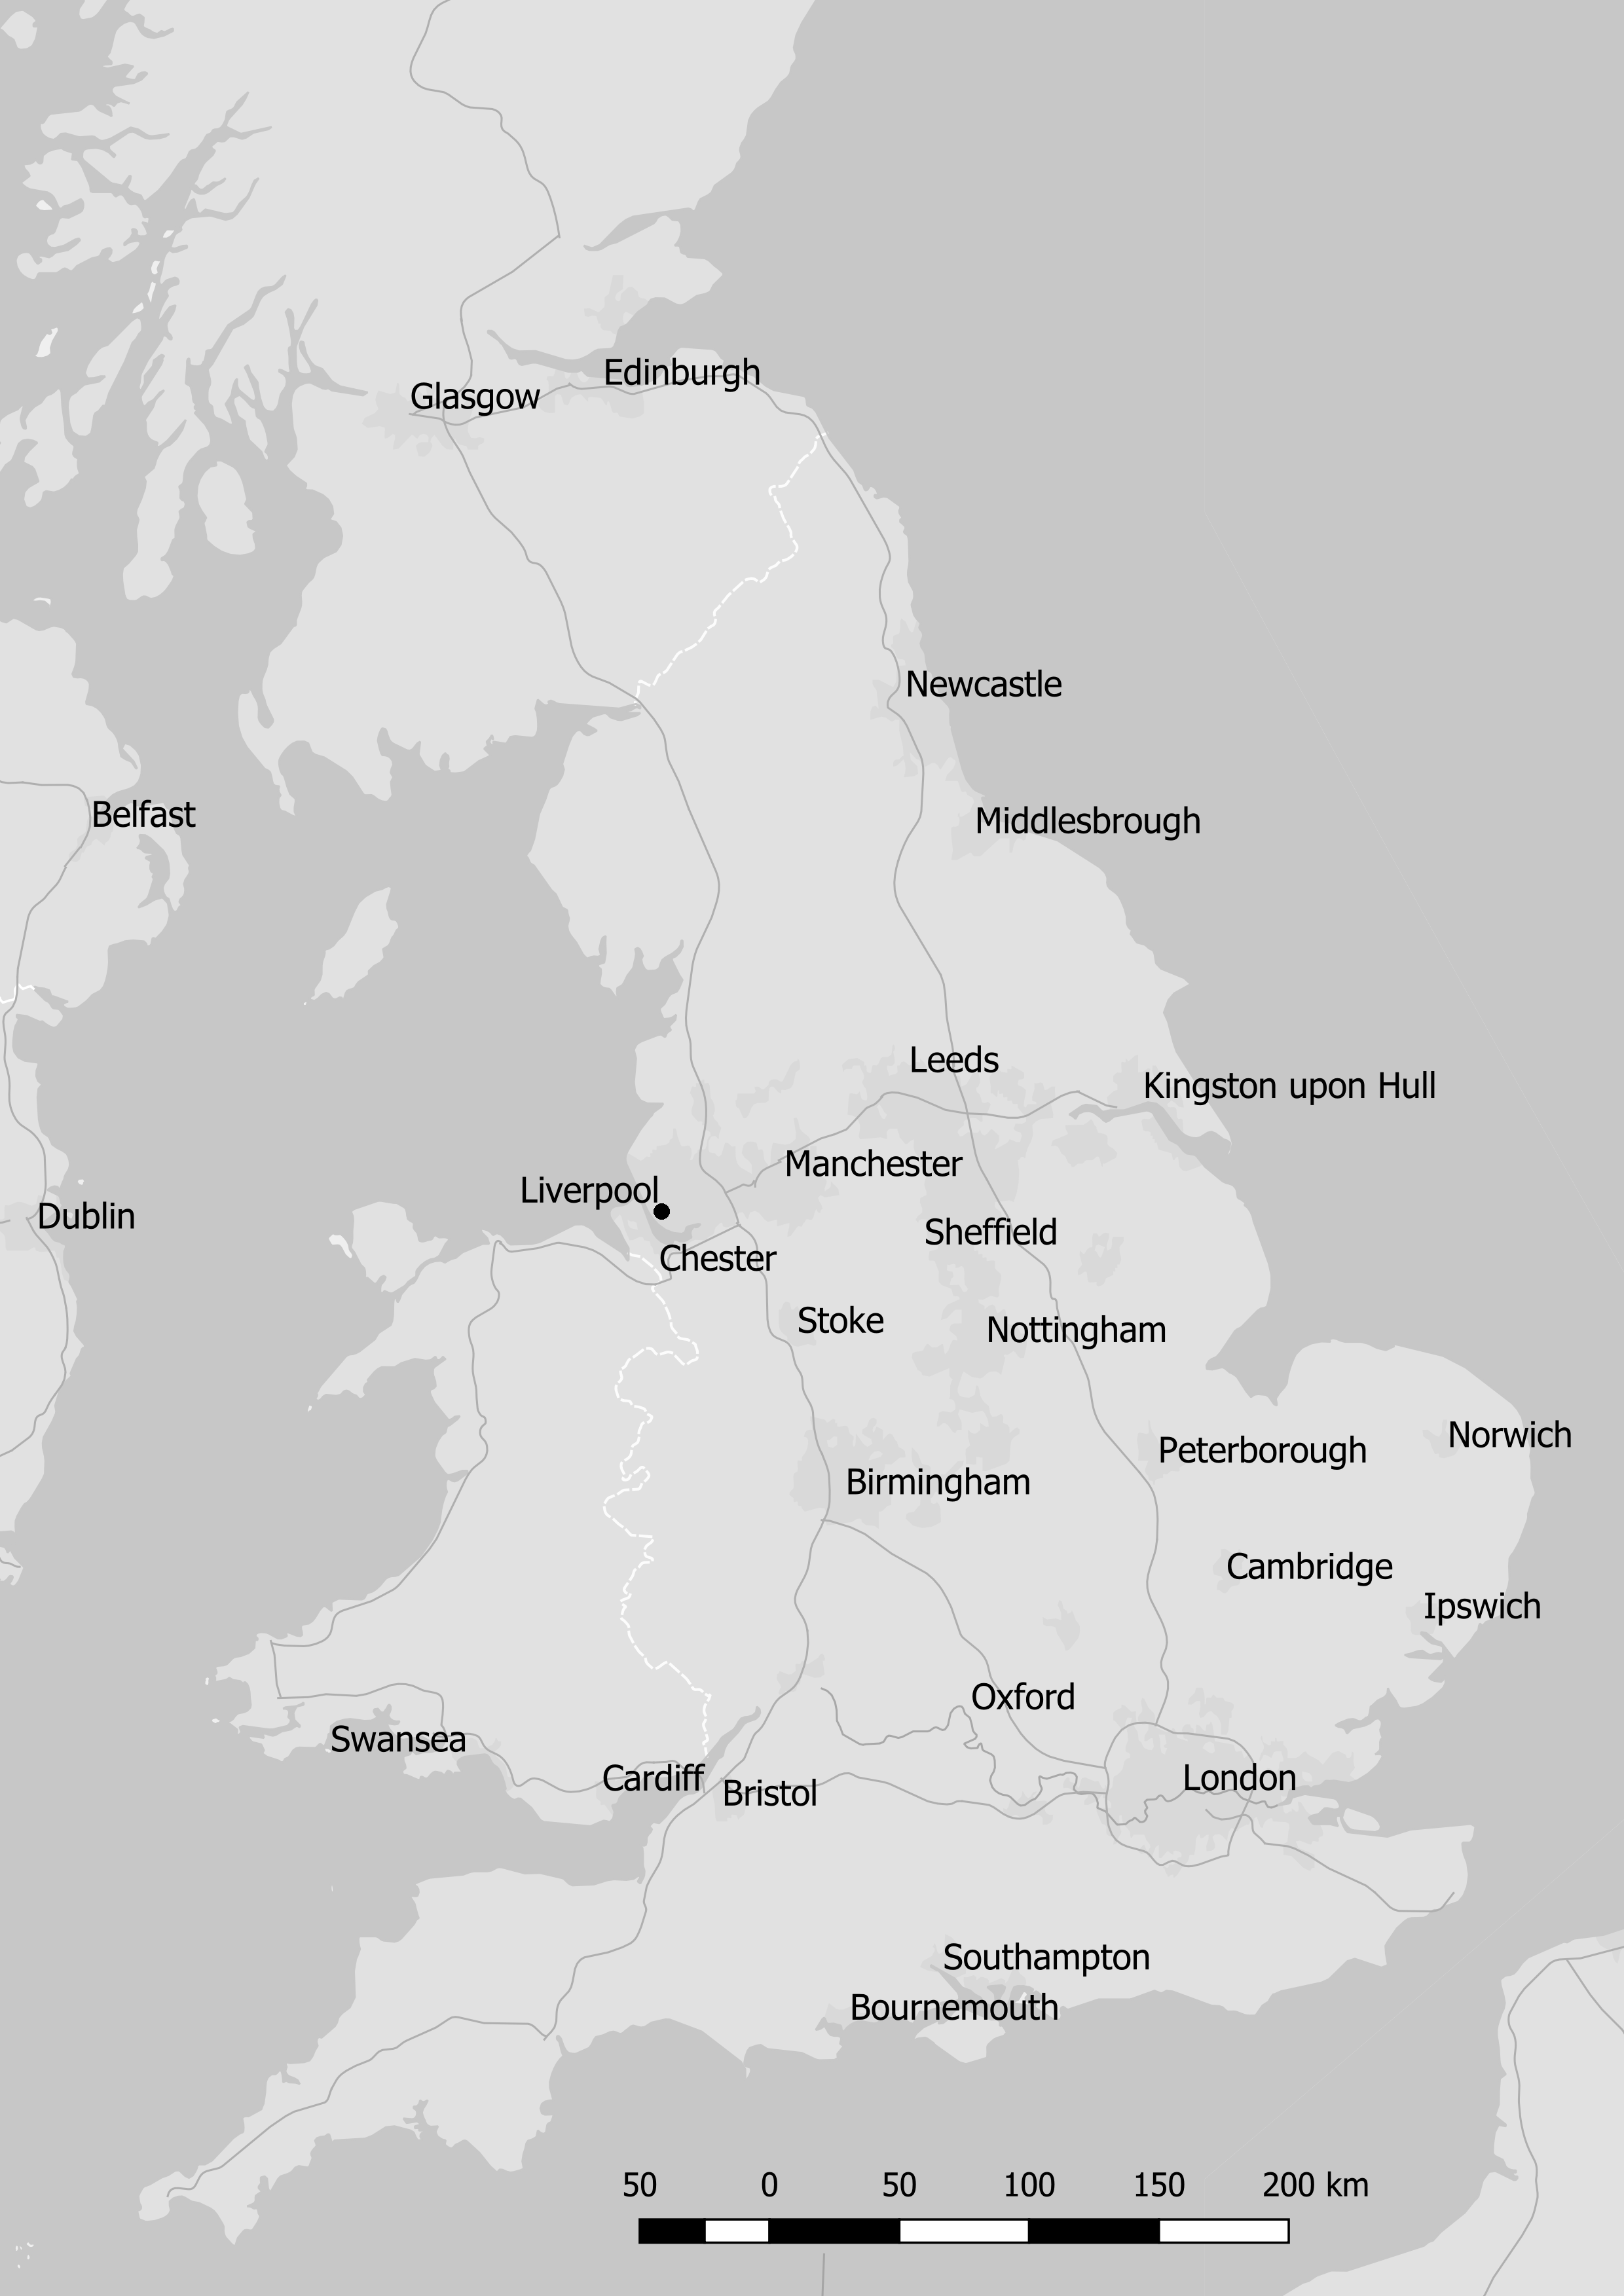
\includegraphics[height=0.4\textheight]{figures/Map-England.png}
		\caption{Liverpool in the UK\\ \tiny Created with \cite{QGIS2016}. Free vector and raster map data @ \url{naturalearthdata.com}}
		\label{fig.ex}
\end{figure}
\clearpage 


In the early 17\textsuperscript{th} century, Liverpool had still not grown beyond its original seven streets, indicating that there was no significant population pressure.
The total population of Liverpool in 1600 is estimated at around 1000 people, making it about the same size as Lancaster or Blackburn, and only between a fifth and a sixth the size of Manchester and Chester.
Commercial activity was modest and remained geographically limited, although Liverpool was already used as a port for exporting \isi{Lancashire} coal, timber, and textiles, and occasional trade with south-western France and northern Spain took place \parencite[cf.][72--76 and 81--84]{kermodeetal2006}.
The latter part of the 17\textsuperscript{th} century saw the establishment and rapid development of new routes, most notably to the West Indies and Liverpool ended up overtaking Chester, which had been the major port of the region until then \citep[cf.][107--110]{kermodeetal2006}.

The general increase in international trade in the second half of the 17\textsuperscript{th} and the first half of the 18\textsuperscript{th} century stimulated growth in all European ports, and in Britain the cities facing west, for obvious reasons, prospered in particular.
Liverpool became the ``focal point'' of a series of road and canal developments in the area, facilitating transport of \isi{Lancashire} coal and \isi{Cheshire} salt to the port \citep[129]{longmore2006}.
The sugar and tobacco trade brought ever greater wealth and a constant flow of work migrants from \isi{Lancashire}, \isi{Cheshire}, North Wales\is{Welsh} and Ireland\is{Irish} to the bustling port on the Mersey.
Between 1700 and 1750 the population trebled to around 18,000, with the majority of the immigrants coming from Liverpool's immediate hinterland \citep[cf.][114--119 and 169]{longmore2006}.

Right from the beginning of the 18\textsuperscript{th} century, Liverpool also participated in one of the most horrible activities of the period: the slave trade.
In fact, Liverpool became ``Britain's leading slave port'' with about 5000 voyages in a little more than 100 years.
While exact figures are difficult to come by, it is estimated that in excess of 40\% of Liverpool's wealth was due to the slave trade.
Expansion was not halted when the slave trade was finally abolished.
Merchants had already diversified their activities, resulting in a thirty-fold increase of Liverpool's tonnage in the 18\textsuperscript{th} century \citep[cf.][131--134 and 137]{longmore2006}.

\largerpage
It can be argued that at the time this enormous commercial success (admittedly only of a wealthy few) ``provided an alternative \isi{identity} for the port'' since Liverpool did not have much of a medieval heritage to draw on (unlike many other provincial towns of the period, e.g. Bristol, Leeds, or Hull).
Despite a rather transitory pattern of residence (even many merchant families only stayed in the city for three generations or less) Liverpool managed to create a perceived ``cultural (\ldots) distinct\is{distinctness}iveness which has arguably remained to the present day''. Due to its international business contacts, the city had a ``cosmopolitan outlook'' and seemed to lie ``outside the culture of \isi{Lancashire}'' \citep[152--154]{longmore2006}.

For \citet[28]{crowley2012} this is actually the point when Scouse as a distinct\is{distinctness}ive variety emerged\is{new-dialect formation}.
Disagreeing with the `received' version of Scouse history that places the beginnings of Scouse in the 19\textsuperscript{th} century (cf. \sectref{sec.hist.19}), he claims that ``given the population statistics, (\dots) it would make more sense to argue that if a new linguistic form was created in Liverpool, then its development surely began (and the form may have even been established) in the eighteenth century''.
His argument is that (in relative terms) the biggest increase in Liverpool's population occurred during this period.
He does acknowledge that most of the people moving into Liverpool in the 18\textsuperscript{th} century came from \isi{Lancashire} but insists that ``the various ports of \isi{Cheshire}, North Wales\is{Welsh} and \isi{Wirral} also contributed, to say nothing of those who migrated from Ireland\is{Irish}, Scotland\is{Scottish}, America and the West Indies''.
\citeauthor{crowley2012} seems to forget for the moment that \isi{Lancashire} and \isi{Cheshire} form a dialect continuum and that the ports of \isi{Cheshire} and the \isi{Wirral} (historically part of \isi{Cheshire} anyway) would therefore not have contributed anything radically different in linguistic terms.
The immediate ``rural hinterland'', however, provided most of the incoming population, particularly at the beginning of the 18\textsuperscript{th} century \parencite[cf.][119]{longmore2006}.

Although the city did indeed continue to grow exponentially (around 77,000 inhabitants by 1800) and notwithstanding its `cosmopolitan outlook', the population of Liverpool remained rather `un-exotic'.
For instance, very few slaves were brought back to Liverpool and those that were sadly died ``almost entirely'' as ``young men, young women and children''.
\textcite[cf.][161 and 169]{longmore2006} further notes that, these few exceptions aside, there seems to be little evidence of a black presence at the time and the current black community therefore must have been established later. \textcite{belchemmacraild2006}, on the other hand, maintain that by the late 1700s a ``vibrant black community'' had developed. However, this community seems to have been very small -- contemporary comments mention only 50 black and mixed-race children in 1787 \parencite[324]{belchemmacraild2006}.

\textcite{crowley2012} also provides some textual evidence for his claim. One of his sources is an early 19\textsuperscript{th} century historian who -- in \citeauthor{crowley2012}'s words -- asserts that ``the \isi{Irish} presence in Liverpool not only grew [in the 18\textsuperscript{th} century], it also contributed to the formation of a distinct\is{distinctness}ive local culture'' \citeyearpar[30]{crowley2012}.
However, the source does not mention accent or dialect in any way, but rather talks about ``local manners in the town'' such as ``hospitality, activity and sprightliness'' (\citealt{troughton1810}, cited in \citealt[30]{crowley2012}).
Another piece of evidence is a play first published and perform\is{accent performance}ed in Liverpool in 1768.
In this play a doctor from Liverpool is urged not to forget the `\isi{Lancashire} dialect' when impersonating a cousin from outside the city.
\citeauthor{crowley2012}'s point is that this should be seen as evidence for the fact that ``the speech of at least some of the inhabitants of Liverpool was not the same as that of Lancastrians'' \parencite[cf.][32--35]{crowley2012}.

This is hardly hot news.
After all, given the language-related ideology already in place at the time -- as \citeauthor{crowley2012} himself points out \citeyearpar[23]{crowley2012} -- no-one would expect a doctor, a well-respected and educated member of the middle class, to use a pronounced regional accent.
The passages that \citeauthor{crowley2012} quotes merely indicate that middle-class Liverpudlians were not speaking with a broad \isi{Lancashire} accent, not that they had developed their own.
To be fair, \citeauthor{crowley2012} himself remarks on the fact that his textual evidence -- just like that of the proponents of the `received version' -- is rather thin.
It appears even less convincing if one considers that, according to oral historians, ``many working-class Liverpudlians failed to exhibit any `scouse' (sic) characteristics (\ldots) in their speech until well into the twentieth century''  \citep[43--44]{belchem2006d} -- more than 100 years after the variety had been coined, if \citeauthor{crowley2012} is correct.


	\section{19\textsuperscript{th} century}\label{sec.hist.19}

From a linguist's point of view, the situation in Liverpool really starts to get interesting in the 19\textsuperscript{th} century, but not much before -- although we have seen above that there is at least one scholar who disagrees with this `received' version of the history of Scouse.
It is, however, generally agreed that Liverpool English is ``a relatively new variety of English'' where ``[a]ll the evidence'' suggests emergence ``from a dialect mixture\is{new-dialect formation}'' \citep[113 and 121]{honeybone2007}.
\citeauthor{honeybone2007} distinguishes three stages in the development of the ``perceptually distinct\is{distinctness} Liverpool English that now exists (\dots)'' \citeyearpar[119]{honeybone2007}:

	\begin{description}
		\item[Stage 1] Broadly pre-19th century
		\item[Stage 2] (Especially mid-) 19th century
		\item[Stage 3] Broadly post-19th century
	\end{description}

He further states that stage 2 is the period ``when the available evidence indicates that the variety came into being'', at a time ``when speakers of a number of dialects were mixing\is{new-dialect formation} in the area'' \parencite[106--107]{honeybone2007}.
And speakers of a number of dialects certainly did mix\is{new-dialect formation} in Liverpool in the 19\textsuperscript{th} century.
From 1801 to 1901, the population increased almost nine-fold -- from around 82,000 to 711,000 \parencite{gbhistgis}.
This, in itself, is nothing out of the ordinary.
Most major cities in Britain, as in other industrialised countries, exploded during the Victorian era.
Manchester, for instance, also went from 88,000 in 1801 to 642,000 in 1901 \parencite{gbhistgis}.
An additional factor is important to understand Liverpool's particular development at the time.

In urban geography, cities are often classified according to two theories, the central place model and the network model.
A central place acts as an administrative and economic centre that provides `services' for its hinterland. Classical examples are medieval market towns.
A network city, on the other hand, is a node in an often international system of cities and as such is less dependent on, and in less intense contact with, its hinterland compared to a central place.
Important ports are prime examples of this type of city.
Obviously, the two functions often overlap and many towns or cities are both central places and network cities.
In the north-west, ``Liverpool and Manchester divided the functions of a regional capital'', with Manchester being the ``summit of the array of central places'' and Liverpool fulfilling the function of ``gateway city linking the region to European and trans-Atlantic urban networks'' \citep[188--189]{hohenberglees1985}.

When the slave trade was finally abolished in 1807, Liverpool turned to raw materials such as timber, oils, and especially cotton.
These raw materials, along with ``the plethora of goods demanded by an urbanizing population'' were needed by Liverpool's hinterland, ``the manufacturing powerhouse that was north-west England'' \parencite[258]{milne2006}.
The goods produced in Manchester and the rest of \isi{Lancashire} and \isi{Cheshire} were then exported through Liverpool's port to the four corners of the globe.
Diversity of goods increased and Liverpool turned into one of the 19\textsuperscript{th} century's only two ``general cargo giants'' in Britain \parencite[259]{milne2006}.
New trading contacts were established in India, China, and South America .
Liverpool increasingly felt at the heart of a global maritime network.
At least to a degree this was certainly justified.
After all, it had become the second biggest city and the most important port in the country by 1850 \citep[cf.][113--114]{honeybone2007}.

In addition to its importance as one of the busiest cargo ports in the world, Liverpool also acquired another function.
Around 1850, the city had established itself as the principal emigration port of the Old World (especially for those bound for the United States) and acquired the nickname `the New York of Europe' \parencite[xxvii]{belchem2006c}.
By way of example, \citet[14]{belchem2006a} notes that in 1851 alone, 455 ships sailed from Liverpool to New York, compared to 124 from Le Havre and 132 from Bremen.
He goes on to explain that more than 85\% of the 5.5 million Europeans that emigrated to America between 1860 and 1900 did so from or through Liverpool.
These emigrants, although their presence was usually only transitory, turned Liverpool into a `diaspora space' and further enhanced its ``cosmopolitan complexion'' \parencite[14]{belchem2006a}.

If contemporary commentators are to be believed, immigrants, travellers, and sailors from all around the world were generally given a friendly welcome by the locals.
An anonymous source counts ``[h]ospitality, social intercourse, civility to strangers, and that freedom from local prejudice which is produced by the residence of so great a proportion of strangers'' among the ``very favourable features in the general portrait'' of Liverpool people (\citealt{anon1812}, cited in \citealt[12]{crowley2012}).
Apparently, this hospitality was also extended to visitors of other races.
\citet[13]{belchem2006a} notes that ``[b]lack passengers in transit were delighted by their reception when they ventured into town, even into the established church''.
\textcite{belchem2006d} also cites a contemporary comment from 1907, describing the Pier Head and the central landing-stage as the place where all of Liverpool met either for business or pleasure and that ``encouraged social intermingling'', having the ``appearance of a democratic promenade'' (\citealt{scott1907}, cited in \citealt[45]{belchem2006d}).

Due to these intensive international contacts\is{dialect contact}, \citet[15]{knowles1973} claims that ``[t]he important linguistic ties'' are less with the \isi{Lancashire} hinterland, and more with ``Dublin and London and the whole of the English speaking world''.
He assumes that Scouse emerged\is{new-dialect formation} as a distinct\is{distinctness} variety some time between 1830 and 1889, which ``corresponds with the period of massive immigration from Ireland\is{Irish}'' \parencite[18]{knowles1973} during and after the \isi{Irish} Potato Famine (1845--1852).
He describes Scouse as being a still essentially north-western variety that has been heavily influenced by \isi{Irish} immigrants \parencite[cf.][51]{knowles1973}.
Applying Trudgill's model of new dialect formation \citep{trudgill1986,trudgill2004} to Liverpool, \textcite{honeybone2007} provides similar dates (1841 to 1891) for the emergence of Scouse but is less categorical with respect to the \isi{Irish} role in the matter.
He explains that, somewhat surprisingly, there was no pronounced founder effect privileging north-western English, although clearly no \emph{tabula rasa} situation existed in Liverpool in the 19\textsuperscript{th} century.
At the same time, \isi{Irish} English was not simply transplanted wholesale to Liverpool \citep[cf.][117 and 121]{honeybone2007}.

This is not to say that \isi{Irish} immigrants were \emph{not} a crucial factor in the formation of Liverpool culture and language.
Their sheer number argues against such ideas.
Even before the famine, many \isi{Irish} emigrated to Liverpool, because it was ``the obvious, indeed often unavoidable place to go from Ireland\is{Irish} as it was the main port of Britain on the West coast, facing Ireland\is{Irish}'' \parencite[114]{honeybone2007}.
Many also originally meant to travel to the United States or other places but ended up staying in Liverpool for good  \citep[cf.][117]{honeybone2007}.
As can be observed from \tabref{tab.birthplace} (adapted from \cite[249]{pooley2006}), about one in five Liverpudlians in the middle of the century had been born in Ireland\is{Irish}.
This is a sizeable proportion, and it has to be borne in mind that people with \isi{Irish} ancestry but who had been born in Liverpool are not even included in this count.

	\begin{table}
		
		\caption{Selected birthplaces of Liverpudlians in the 19\textsuperscript{th} century}
		\begin{tabularx}{\textwidth}{Xrrr}
			\lsptoprule
			Birthplace & 1851 & 1871 & 1891 \\ 
			\midrule
			\isit{Lancashire} (including Liverpool)&  {50.3\%} &   {58.7\%} &  {68.9\%} \\ 
			Ireland\is{Irish} & 22.3\% & 15.6\% & 9.1\% \\ 
			Wales\is{Welsh} & 5.4\% & 4.3\% & 3.4\% \\ 
			Scotland\is{Scottish} & 3.7\% & 4.1\% & 3.0\% \\
			\isit{Cheshire} & 3.4\% & 3.0\% & 2.8\% \\ 
			\lspbottomrule
		\end{tabularx}
		\label{tab.birthplace}
	\end{table}

A number of problems arise if one is to take \citeauthor{knowles1973}' view and consider \isi{Irish} English speakers as the dominating influence in the creation of Scouse.
The \isi{Irish} were
\begin{inparaenum}[a\upshape)]
	\item highly concentrated -- one might say ghettoised -- in certain parts of the city, 
	\item ``only ever an absolute majority in few streets'' \citep[120]{honeybone2007}, 
	\item generally of a lower socio-economic status than people born in Liverpool, and
	\item for the most part Roman Catholics \citep[cf.][330]{belchemmacraild2006}.
\end{inparaenum}
These features add up to a spatially isolated and heavily stigmatise\is{stigmatisation}d group of Liverpool society at the time.
Under these circumstances, it is very difficult to argue convincingly that ``their speech would swamp the dialects of inmigrants from other areas'', as \citet[120]{honeybone2007} rightly points out.
What is more, the proportion of \isi{Irish} migrants was similar in other cities.
\citet[140]{honeybone2007} cites 18.1\% and 13.1\% for Glasgow and Manchester in 1851 respectively, so the number of speakers alone cannot account for the particular linguistic development in Liverpool.

\tabref{tab.birthplace} also indicates that there was a non-negligible community of \isi{Welsh} and Scots (more than 9\% in 1851, again not counting second and third generation immigrants).
These figures are small compared to the \isi{Irish} part, but they were still large enough for Liverpool to acquire the nickname `the capital of North Wales\is{Welsh}' and to boast the second-largest Scots community in England.
Neither \isi{Welsh} nor Scots were spatially as concentrated as the \isi{Irish}, although they did constitute what \citeauthor{honeybone2007} calls ``highly organised'', i.e. somewhat inward-look\-ing and self-sufficient, communities \citep[cf.][120--121]{honeybone2007}.
Unlike the \isi{Irish}, these groups were associated with the skilled working population \citep[cf.][202--203]{belchem2006b}, which makes their dialects more likely contributors to the emerging Scouse than the varieties spoken by a non-prestigious group like the \isi{Irish}.
To these larger minorities, one must add smaller numbers of people not represented in \tabref{tab.birthplace} -- from all over Britain, Africa, the Caribbean, and China.
All of these people have, in some way, contributed to the dialect mix\is{new-dialect formation} in the city \citep[cf.][116]{honeybone2007}.

Knowles and Honeybone disagree to an extent about which influences most shaped early Scouse.
However, both assert, the former on the basis of somewhat cryptic comments in \citealt{ellis1889} \citep[cf.][18]{knowles1973}, the latter using Trudgill's new-dialect\is{new-dialect formation} model \citep[cf.][118]{honeybone2007}, that by the end of the 19\textsuperscript{th} century a variety identifiable as `Liverpool English' had emerged.

	\section{20\textsuperscript{th} century}\label{sec.hist.20}

		\subsection{Enregisterment and the `Scouse industry'}\label{sec.hist.20.industry}

Liverpool continued to grow in the 20\textsuperscript{th} century, reaching its population pinnacle of around 855,000 in 1931 \citep[cf.][171]{pooley2006}, despite the fact that Liverpool's economic vulnerability was dramatically revealed during the inter-war years when the world economy slumped and 30\% of port-related jobs disappeared overnight.
The port acquired outstanding, though short-lived, importance again during World War 2 when Liverpool was the European end point of the Allied convoys, as well as the command centre for the Battle of the Atlantic (a fact which also made it a prime target for the Luftwaffe, which wreaked considerable destruction on the city and killed thousands of people in 1940--1941) \citep[cf.][393 and 405]{murden2006}.
While immigration from all parts of the word continued \citep[cf.][119]{honeybone2007}, attitudes towards migrants became less positive, at least in some parts of Liverpool society.
At times ``hysterical reaction[s]'' in the local press can now be seen as precursors of the ``troubled pattern of `racialized relations''' in the latter part of the 20\textsuperscript{th} century \citep[cf.][23]{belchem2006a}.

At around the same time (the early to mid-20\textsuperscript{th} century) developed what \citet[40]{crowley2012} calls the ``\isi{Scouse industry}''.
From the 1930s onwards, a number of articles and letters to the editors in local newspapers discussing `Liverpool' words and phrases can be found.
While most of these claims were incorrect -- \citet[48]{knowles1973} comments on ``the very paucity of the material'' particular to Scouse in the domain of grammar and vocabulary -- they nevertheless ``indicated that there was a developed sense that Liverpool as a place had a vocabulary (and a mode of pronunciation) that was part of its cultural distinct\is{distinctness}iveness within Britain'' \parencite[42]{crowley2012}.
In other words, \emph{\isi{enregisterment}} was well under way, and Scouse was turning -- or had already turned -- into a ``socially recognised register of forms'' that was ``differentiable within [the] language'' \parencite[231]{agha2003}.
In the years following World War 2, two individuals in particular gained publicity in this domain and are still well-known today.
Neither Frank Shaw nor Fritz Spiegl were linguists (Shaw worked as a customs officer, Spiegl was a flutist), but rather amateurs (in the original sense) who ran a campaign to ``present Scouse as the language of Liverpool'' and who tried to ``popularize, celebrate and preserve aspects of the language and culture of Liverpool'' \citep[64--65]{crowley2012}.
The \emph{Lern Yerself Scouse} series sparked off by these two in the 60s can still be found in most Liverpool book shops today.
On the surface at least, these short booklets were intended as a sort of phrasebook for visitors of the city, familiarising them with vocabulary and pronunciations peculiar (in the authors' opinion) to Liverpool English. \citet{honeybonewatson2013} provide a linguistic analysis of these volumes (cf. also Chapter \ref{ch.var}).

Although the series may well be considered ``the touchstone for the \isi{Scouse industry}'' \citep[79]{crowley2012}, it was clearly not its only manifestation.
As early as the 1930s, the city had established for itself a ``reputation for humour'' that was carried on in the 1960s by comedians such as Ken Dodd and Jimmy Tarbuck, both in theatres across the country and on TV (cf. \citealt[423]{murden2006}, and \citealp[49]{belchem2006a}).
Liverpool was also represented on national TV in the 1950s and 60s with series like \emph{Z-Cars} or \emph{The Liver Birds}, which showed characters that ``often conformed to the cultural, linguistic and social representations that had been set out by the founders of the \isi{Scouse industry}'' \parencite[75]{crowley2012}.
Finally, numerous pop bands came out of Liverpool during the Merseybeat era, the most famous and influential of which was the Beatles.
They acquired unprecedented fame for Liverpool and, at least for a couple of years, made the city the centre of the pop music world \citep[cf.][75]{crowley2012}, while ``Britain fell in love with everything connected to Liverpool'' \citep[423]{murden2006}.

Based on his textual/literary evidence, \citet[107]{crowley2012} claims that the stage of ``first-order (sic) \isi{indexicality} with regard to Liverpool speech'' was reached ``in the early to mid twentieth century''.
His argument is that ``there is clear evidence that words and sounds were postulated (often incorrectly) as belonging uniquely to Liverpool''.
Since these postulations stem from non-experts, however, we are at this point dealing with third-order \isi{indexicality} already, since the peculiarities have started attracting explicit comment.
This must be a typographical error, otherwise \citeauthor{crowley2012}'s claim is even more strange if we remember him arguing elsewhere that Scouse had already emerged from dialect-mixing\is{new-dialect formation} in the 18\textsuperscript{th} century (cf. \sectref{sec.hist.early}).
Based on \citeauthor{silverstein2003}' \citeyear{silverstein2003} orders of \isi{indexicality}, \textcite[81]{johnstoneetal2006} define first-order \isi{indexicality} as ``the kind of correlation between a form and a sociodemographic \isi{identity} (\ldots) that an outsider could observe'', i.e. experts can identify a feature as being indicative of a particular group of speakers, possibly even while the variety is still emerging.
Crucially, however, this features does not yet do social work (second-order \isi{indexicality}), nor is it talked about or used in conscious\is{awareness} perform\is{accent performance}ances (third-order \isi{indexicality}) of local \isi{identity} \parencite[cf.][83--84]{johnstoneetal2006}.

Nevertheless, \citeauthor{crowley2012} correctly explains that the comments by Shaw and others, distinguishing `real Liverpudlian\is{identity}s' from `middle-class Mossley Hill Liverpolitans', to use Shaw's phrasing, indicate (at least) second-order \isi{indexicality}. Social stratification\is{social stratification} was, apparently, firmly in place with respect to Liverpool English, which is why it had already become ``the index not simply of Liverpool \isi{identity}, but of Liverpool working-class \isi{identity}'' \citep[107]{crowley2012}.
When some features of Scouse definitely reached third-order \isi{indexicality} in the 1960s, this association with the working-class was less of a problem than several decades before and might even have contributed to the `coolness' (The `Liverpool cult' -- \citealt[109]{crowley2012}) of Scouse \isi{identity}.
As \citet[165]{wales2006} notes, ``it became fashionable to be young, working class and urban, and the importance of this on language \isi{change} in the late twentieth century should not be underestimated''.

		\subsection{Decline}\label{sec.hist.20.decline}
\largerpage[-1]
While Liverpool was enjoying its heyday in terms of \isi{image} and popularity, it was already facing serious difficulties in other respects. After a short revival in the 1950s \citep[cf.][402]{murden2006}, economic decline hit the city hard from the 1960s and especially the 1970s onwards.
Following the 1973 oil crisis, most western countries went into recession and thousands of manufacturing jobs were lost.
While new service jobs countered this loss, they usually developed in other regions (in the case of Britain, in the south of England) than those most affected by structural \isi{change} (here northern England) \citep[cf.][16--17]{juddparkinson1990a}.

Liverpool had prospered enormously as a trading hub in the Victorian era, but the end of the British Empire, the ``collapse of the colonial economic system'' \citep[52]{belchem2006a}, and Britain's (economic) shift of focus towards Europe meant that Liverpool ``found itself poorly located to take advantage of the increasing trade between the UK and mainland Europe'' that now dominated \citep[166--167]{couch2003a}.
In addition, containerisation meant that even the few ports that were able to retain their importance (Rotterdam and Hamburg alone ended up serving all of northern Europe, cf. \citealt[264]{milne2006}) no longer required thousands of workers, but just a handful of more specialised employees to operate the machinery.
Due to its container terminal in Seaforth, Liverpool's port today handles more cargo than ever before, but it does so with a workforce of only 800 (7000 in the whole maritime sector; figures for 2003, \citealt[cf.][477]{murden2006}).

The central government tried to fight unemployment by encouraging private investors to open up new factories in the city, but in most cases success was short-lived.
The militancy of Liverpool workers -- ``a myth in the making'' -- was often used as a pretext whenever \isi{Merseyside} plants were the first to be closed again ``[o]nce development aid and other short-term advantages were exhausted''\citep[cf.][52]{belchem2006a}.
Liverpool became the ``beaten city'' and a ```showcase' of everything that has gone wrong in Britain's major cities'' \citep[\emph{Daily Mirror}, 11 October 1982, cited in][52--53]{belchem2006a}.

While claims concerning the militancy of Liverpudlian\is{identity}s in general might well have been more based on \isi{stereotype}s than fact, there certainly was \emph{political} militancy in the form of Militant Tendency (a Labour `sect') in the 1980s.
Until 1979, central government measures were focused on social and welfare services on the one hand and the creation of public sector jobs on the other. When Margaret Thatcher became prime\is{priming} minister, however, urban policy changed \citep[cf.][19]{juddparkinson1990a}.
Public spending was to be cut back considerably.
The Militant majority of Liverpool City Council disagreed and, in the eyes of some at least, tried to \enquote{force} the government into granting them additional funds and effectively ``threaten[ed] to bankrupt the city if it were not given the extra resources''.
In 1987 the House of Lords finally disqualified 47 Labour officials of the City Council from office for failing to protect the financial interest of the city \citep[cf.][249--250]{parkinson1990}.
But the damage had been done.
Liverpool's ``political failure'' \citep[241]{parkinson1990} resulted in a ``sharp decline in investor confidence'' and a ``deterioration in the \isi{image} of the city'' which lasted for many years \citep[172]{couch2003a}.

Economic decline was followed by physical deterioration.
In the 1980s, Central Liverpool was fast losing population and jobs, the shopping centre had to yield business to retail parks in the suburbs, congestion was on the rise and environmental conditions went downhill \citep[cf.][38]{couch2003}.
This ``visual legacy of dereliction'' brought with it an ``air of decay'' which made the area even less attractive to potential private sector investors and thereby created or at least contributed to a downward spiral of recession and decay \citep[21]{fraser2003}.
 
Due to these economic problems (and the limited opportunities for migrants that ensued), Liverpool did not participate in the post-war mass-immigration from the Caribbean and South Asia in the same way as other major British cities did.
While Liverpool was, after London, the most ethnically diverse British city in the 19\textsuperscript{th} century, it is clear from \tabref{tab.ethnicity} (data are from \citealt{nomis}) that this is no longer true.
In fact, although minorities now make up a larger proportion of Liverpool residents than in 2001 (largely due to a recent influx of refugees and asylum seekers), it is today still one of the \emph{least} ethnically diverse places in Britain, clearly lagging behind Manchester in this respect and a far-cry from places such as Birmingham or London \citep[cf.][187]{pooley2006}.

	\begin{table}[h]
		
		\caption{Ethnicity in Liverpool and other major cities (\%)}
		\begin{tabular}{lrrrrrrrr}
			\lsptoprule
	 		& \multicolumn{2}{c}{Liverpool} & \multicolumn{2}{c}{Manchester} & \multicolumn{2}{c}{Birmingham} & \multicolumn{2}{c}{London} \\
			 & 2001 & 2011 & 2001 & 2011 & 2001 & 2011 & 2001 & 2011 \\
			 \midrule
			 white & 94.32 & 88.91 & 80.96 & 66.61 & 70.35 & 57.93 & 71.15 & 59.79 \\
			 black & 1.22 & 2.64 & 4.51 & 8.64 & 6.12 & 8.98 & 10.92 & 13.32 \\
	 		 Asian & 2.27 & 4.16 & 10.44 & 17.09 & 20.04 & 26.62 & 13.20 & 18.49 \\
	 		 mixed & 1.80 & 2.52 & 3.23 & 4.60 & 2.86 & 4.44 & 3.15 & 4.96 \\
	 		 other & 0.39 & 1.77 & 0.86 & 3.06 & 0.63 & 2.03 & 1.58 & 3.44 \\
	 		 \lspbottomrule
		\end{tabular}
		\label{tab.ethnicity}
	\end{table}

In addition, Liverpool's minority population is (and always has been) highly concentrated (segregated?) in central areas of the city.
Furthermore, the ``most visible'' minorities -- especially blacks and Chinese -- had to endure marginalisation and a certain degree of racial violence from the early 20\textsuperscript{th} century onwards \citep[cf.][189--191]{pooley2006}.
Racial tensions and more general disappointment with the authorities culminated in the Toxteth riots of 1981, which lasted for two weeks, caused \pounds11 million of damage, and left hundreds of people (police and civilians) injured and one dead \citep[cf][440--444]{murden2006}.

All of this had an impact on evaluations of the primary expression of Liverpool culture, Scouse.
Scouse had received poor popular ratings already in the 1970s and these results were corroborated in a 1990s survey where Scouse got an approval rating of only 6\%, while at the same time frequently joining other northern accents in scoring rather highly for `friendliness' \citep[cf.][166]{wales2006}.
What is even more important than the negative \emph{external} perceptions of Liverpool and Scouse is what \citet[255]{parkinson1990} calls an ``internal \isi{image} problem''.
Writing in \citeyear{parkinson1990}, he claims: 
	\begin{quote}
		Two decades of economic failure, compounded by political failure and self-destruction, have bred a degree of cynicism in the city's public life. There is clearly a cultural dimension to the city's failure that goes beyond the statistics of economic decline.
	\end{quote}

 
It probably goes without saying that this ``cultural dimension'' is highly likely to also include the linguistic domain.
It would not be surprising if an ``internal \isi{image} problem'' impacted on people's (socio-)linguistic behaviour, i.e. if at least some speakers tried to tone down their local accent a bit because they felt it to be somewhat contaminated by the negative associations attached to the city.
If this was the case then it may well have helped bring about, or at least accelerate, what \citet{knowles1978} calls the `extensive standardisation' of Scouse in the 20\textsuperscript{th} century.

		\subsection{Regeneration}\label{sec.hist.20.regen}

Politicians in Liverpool and London did not just passively watch the city's physical decline.
Post-war measures mostly focused on public housing, inner city slum clearance and relocation of the population to new housing estates on the periphery.
From the beginning of the 1980s, the strategy slowly started to change.
The emphasis shifted to the ``potential of the city center in terms of retail, leisure, tourism, and commercial development''.
The city council even funded studies evaluating the tourist potential and dealing with issues such as Liverpool's negative \isi{image} and city marketing \citep[cf.][250--253]{parkinson1990}.

Decline continued all the same, and in 1993 Liverpool (and the whole region of \isi{Merseyside} to be exact) had spiralled down into Objective One status -- a label given by the EU to regions whose GDP per capita is 75\% or less of the EU average.
\citet[53--54]{belchem2006a} notes that ``[a]lthough at the time it seemed a badge of failure'' this may well turn out to have been a ``decisive turning point for the city'', because it gave access to considerable European funds.
In its wake, the city council turned towards ``urban entrepreneurialism, partnership governance and civic boosterism'', which is very unlike the political style that was prevalent in the 1980s.

\largerpage
Economically, it had become clear, in Liverpool and elsewhere, that it was not possible to recreate the past.
Instead, the future was envisaged in information technology and new (tertiary) industries, such as banking and advertising \citep[cf.][32]{fraser2003}.
A local film industry was also successfully established in the second half of the 1980s and 1989 saw the creation of the Liverpool Film Office, the first of its kind in the UK \citep[cf.][479]{murden2006}.
First and foremost, however, Liverpool turned towards tourism and (re-)discovered its cultural heritage as an economic asset \citep[cf.][32--33]{fraser2003}.
The city centre was physically improved through, for example, new squares, public spaces, and pedestrianised shopping areas.
The waterfront, with its unused docks and warehouses, has proved particularly suitable for regeneration as a tourist and leisure area \citep[173--174]{couch2003a}.

Regeneration did (and does) also face problems.
Just as in other places in the UK, the ``private development sector'' is rather powerful.
As a consequence, most measures have focused on high-return investments in the city centre with an ensuing neglect of more peripheral areas, such as Vauxhall or North Liverpool, that are just as much (or even more) in need of regeneration \citep[cf.][49]{couch2003}.
Furthermore, Liverpool is in competition with Manchester, which is now the undisputed regional capital thanks to its airport (the most important one outside London) and its more central location.
As such, Manchester was (and still is) often the more obvious choice for potential investors in the north-west.
While the ``deep-seated social and economic problems (\ldots) still remain acute'' \citep[188]{fraser2003a}, it is nonetheless important to remember that ``a great deal [was achieved], at least in terms of physical \isi{change}'' \citep[44]{couch2003}.

Due to the fact that private investors were now operating on an international level, it became important for cities to emphasise their local attributes through the use of place promotion and marketing strategies.
Cultural revitalisation, organisations like Liverpool Vision and \isi{prestige} projects such as the Albert Dock are examples of this attempt to create and foster a new \isi{image}.
In addition to attracting investment, these projects can also instil pride into local people and thus ``help to promote civic \isi{identity}'' \citep[cf.][201--203]{percy2003}.

Pride in the city is an important aspect.
\citet[20]{fraser2003} explains that cities past their heyday such as Liverpool ``should be vanishing as new centres [take] their place''.
Obviously, this is not what has happened.
Rather, people try ``to find a new rationale for its existence and re-creation of its former prosperity. \emph{It is a matter of conscious\is{awareness} choice to do so}'' (my emphasis).
This conscious\is{awareness} choice not to give up is, among other things, based on ``a \emph{sense of place}, a special character or feeling in and for that place, which attracts loyalty from inhabitants'' \citep[23, emphasis in the original]{fraser2003}.
Successful regeneration might well have filled Liverpudlian\is{identity}s with new self-pride and self-respect.
New self-respect in turn should manifest itself in (sub-)conscious\is{awareness} reinforcement of social \isi{marker}s such as accent.


We might even suspect that the external \isi{image} of Scouse has also improved.
If \citet[73]{trudgill1999} and \citet[110]{honeybone2007} are to be believed, Scouse must have acquired some covert \isi{prestige} by the late 1990s and spread not only to Birkenhead, but also to more rural areas in \isi{Merseyside}.
\citet[176--177]{montgomery2007a} even -- speculatively -- suggests that some people from Crewe in \isi{Cheshire} might identify with Scouse.
The fact that a great number of new call centres were established in \isi{Merseyside} in 1998 also casts some doubt on ``the usual stigma attached to Scouse'' as ``[t]elesales companies have apparently taken great care to locate their call centres in regions where their workers' accents will be favourably perceived'' \citep[3]{foulkesdocherty1999a}.

	\section{21\textsuperscript{st} century -- outlook}\label{sec.hist.21}

Regeneration continued into the new millennium with the construction of a new big convention centre (the Echo Arena) and the transformation of RopeWalks into a modern, trendy leisure quarter housing a media arts centre and numerous bars, restaurants, and clubs.
In the very centre of the city, about £920 million were spent on Liverpool ONE, one of the largest open-air retail spaces in the UK, but also comprising residential and leisure facilities.
From 2004 to 2008 it completely transformed about 42 acres of previously rather bleak land and, in passing, considerably improved access to the city centre by public transport thanks to the new bus interchange that was part of the project \parencite[cf.][478--479]{murden2006}.
An even bigger development project, Liverpool Waters, was granted planning permission in March 2013 and is supposed to create 17,000 jobs while redeveloping the north docks.

Liverpool also continued to do well on the culture front.
In 2004, parts of the waterfront and the Cultural Quarter (the area around St. George's Hall and the World Museum) were inscribed on UNESCO's list of World Heritage Sites, a badge which surely further increased Liverpool's attraction as a tourist destination.
Probably the most important achievement of the city in the new millennium so far is its success in acquiring the title of European Capital of Culture in 2008 (together with Stavanger in Norway).
Not only did this title provide the occasion and the framework for a year of events and festivals, it also had a number of measurable effects.
As a direct consequence of the title, around 9.7 million additional visitors were counted in 2008, with 97\% of the international tourists visiting for the first time.
More than £750 million of direct income for the city's economy was created this way, and data collected from 2005 to 2010 indicate that the `Capital of Culture' effect could be lasting \parencite{garciaetal2010}.
In the long term, what may be even more important is that media coverage has also \isi{change}d.
In the 1990s national media largely focused on (usually negative) social issues when covering Liverpool, while in 2008/2009 ``culture and \isi{image} stories'' dominated.
Local media also showed a pronounced increase in positive coverage in the years leading up to 2008 as well.
Positive impressions about Liverpool increased statistically significantly in national surveys from 2005 to 2008 \citep[cf.][25 and 44--46]{garciaetal2010}.

	\begin{figure}
		
		% Created by tikzDevice version 0.10.1 on 2017-03-14 14:20:47
% !TEX encoding = UTF-8 Unicode
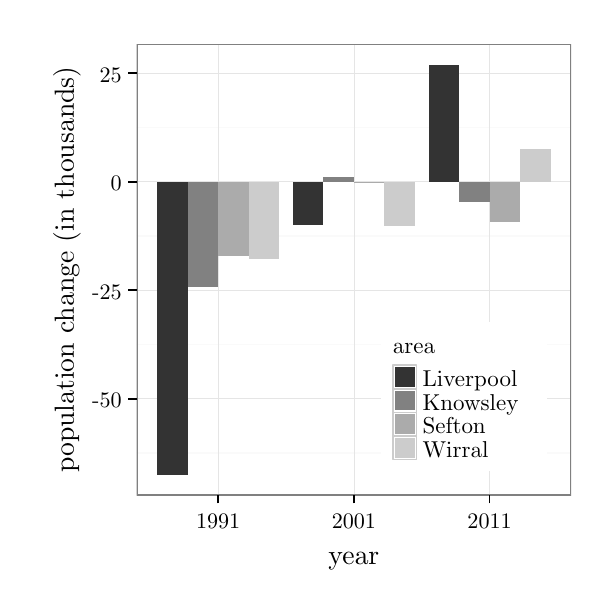
\begin{tikzpicture}[x=1pt,y=1pt]
\definecolor{fillColor}{RGB}{255,255,255}
\path[use as bounding box,fill=fillColor,fill opacity=0.00] (0,0) rectangle (202.36,202.36);
\begin{scope}
\path[clip] (  0.00,  0.00) rectangle (202.36,202.36);
\definecolor{drawColor}{RGB}{255,255,255}
\definecolor{fillColor}{RGB}{255,255,255}

\path[draw=drawColor,line width= 0.6pt,line join=round,line cap=round,fill=fillColor] (  0.00,  0.00) rectangle (202.36,202.36);
\end{scope}
\begin{scope}
\path[clip] ( 39.40, 33.48) rectangle (196.36,196.36);
\definecolor{fillColor}{RGB}{255,255,255}

\path[fill=fillColor] ( 39.40, 33.48) rectangle (196.36,196.36);
\definecolor{drawColor}{gray}{0.98}

\path[draw=drawColor,line width= 0.6pt,line join=round] ( 39.40, 48.66) --
	(196.36, 48.66);

\path[draw=drawColor,line width= 0.6pt,line join=round] ( 39.40, 87.87) --
	(196.36, 87.87);

\path[draw=drawColor,line width= 0.6pt,line join=round] ( 39.40,127.08) --
	(196.36,127.08);

\path[draw=drawColor,line width= 0.6pt,line join=round] ( 39.40,166.29) --
	(196.36,166.29);
\definecolor{drawColor}{gray}{0.90}

\path[draw=drawColor,line width= 0.2pt,line join=round] ( 39.40, 68.27) --
	(196.36, 68.27);

\path[draw=drawColor,line width= 0.2pt,line join=round] ( 39.40,107.48) --
	(196.36,107.48);

\path[draw=drawColor,line width= 0.2pt,line join=round] ( 39.40,146.69) --
	(196.36,146.69);

\path[draw=drawColor,line width= 0.2pt,line join=round] ( 39.40,185.90) --
	(196.36,185.90);

\path[draw=drawColor,line width= 0.2pt,line join=round] ( 68.83, 33.48) --
	( 68.83,196.36);

\path[draw=drawColor,line width= 0.2pt,line join=round] (117.88, 33.48) --
	(117.88,196.36);

\path[draw=drawColor,line width= 0.2pt,line join=round] (166.93, 33.48) --
	(166.93,196.36);
\definecolor{fillColor}{gray}{0.20}

\path[fill=fillColor] ( 46.76, 40.88) rectangle ( 57.79,146.69);
\definecolor{fillColor}{RGB}{129,129,129}

\path[fill=fillColor] ( 57.79,108.83) rectangle ( 68.83,146.69);
\definecolor{fillColor}{gray}{0.67}

\path[fill=fillColor] ( 68.83,119.87) rectangle ( 79.87,146.69);
\definecolor{fillColor}{gray}{0.80}

\path[fill=fillColor] ( 79.87,118.63) rectangle ( 90.90,146.69);
\definecolor{fillColor}{gray}{0.20}

\path[fill=fillColor] ( 95.81,130.96) rectangle (106.84,146.69);
\definecolor{fillColor}{RGB}{129,129,129}

\path[fill=fillColor] (106.84,146.69) rectangle (117.88,148.24);
\definecolor{fillColor}{gray}{0.67}

\path[fill=fillColor] (117.88,146.56) rectangle (128.91,146.69);
\definecolor{fillColor}{gray}{0.80}

\path[fill=fillColor] (128.91,130.53) rectangle (139.95,146.69);
\definecolor{fillColor}{gray}{0.20}

\path[fill=fillColor] (144.85,146.69) rectangle (155.89,188.95);
\definecolor{fillColor}{RGB}{129,129,129}

\path[fill=fillColor] (155.89,139.53) rectangle (166.93,146.69);
\definecolor{fillColor}{gray}{0.67}

\path[fill=fillColor] (166.93,132.29) rectangle (177.96,146.69);
\definecolor{fillColor}{gray}{0.80}

\path[fill=fillColor] (177.96,146.69) rectangle (189.00,158.45);
\definecolor{drawColor}{gray}{0.50}

\path[draw=drawColor,line width= 0.6pt,line join=round,line cap=round] ( 39.40, 33.48) rectangle (196.36,196.36);
\end{scope}
\begin{scope}
\path[clip] (  0.00,  0.00) rectangle (202.36,202.36);
\definecolor{drawColor}{RGB}{0,0,0}

\node[text=drawColor,anchor=base east,inner sep=0pt, outer sep=0pt, scale=  0.80] at ( 34.00, 64.96) {-50};

\node[text=drawColor,anchor=base east,inner sep=0pt, outer sep=0pt, scale=  0.80] at ( 34.00,104.17) {-25};

\node[text=drawColor,anchor=base east,inner sep=0pt, outer sep=0pt, scale=  0.80] at ( 34.00,143.38) {0};

\node[text=drawColor,anchor=base east,inner sep=0pt, outer sep=0pt, scale=  0.80] at ( 34.00,182.59) {25};
\end{scope}
\begin{scope}
\path[clip] (  0.00,  0.00) rectangle (202.36,202.36);
\definecolor{drawColor}{RGB}{0,0,0}

\path[draw=drawColor,line width= 0.6pt,line join=round] ( 36.40, 68.27) --
	( 39.40, 68.27);

\path[draw=drawColor,line width= 0.6pt,line join=round] ( 36.40,107.48) --
	( 39.40,107.48);

\path[draw=drawColor,line width= 0.6pt,line join=round] ( 36.40,146.69) --
	( 39.40,146.69);

\path[draw=drawColor,line width= 0.6pt,line join=round] ( 36.40,185.90) --
	( 39.40,185.90);
\end{scope}
\begin{scope}
\path[clip] (  0.00,  0.00) rectangle (202.36,202.36);
\definecolor{drawColor}{RGB}{0,0,0}

\path[draw=drawColor,line width= 0.6pt,line join=round] ( 68.83, 30.48) --
	( 68.83, 33.48);

\path[draw=drawColor,line width= 0.6pt,line join=round] (117.88, 30.48) --
	(117.88, 33.48);

\path[draw=drawColor,line width= 0.6pt,line join=round] (166.93, 30.48) --
	(166.93, 33.48);
\end{scope}
\begin{scope}
\path[clip] (  0.00,  0.00) rectangle (202.36,202.36);
\definecolor{drawColor}{RGB}{0,0,0}

\node[text=drawColor,anchor=base,inner sep=0pt, outer sep=0pt, scale=  0.80] at ( 68.83, 21.47) {1991};

\node[text=drawColor,anchor=base,inner sep=0pt, outer sep=0pt, scale=  0.80] at (117.88, 21.47) {2001};

\node[text=drawColor,anchor=base,inner sep=0pt, outer sep=0pt, scale=  0.80] at (166.93, 21.47) {2011};
\end{scope}
\begin{scope}
\path[clip] (  0.00,  0.00) rectangle (202.36,202.36);
\definecolor{drawColor}{RGB}{0,0,0}

\node[text=drawColor,anchor=base,inner sep=0pt, outer sep=0pt, scale=  1.00] at (117.88,  8.40) {year};
\end{scope}
\begin{scope}
\path[clip] (  0.00,  0.00) rectangle (202.36,202.36);
\definecolor{drawColor}{RGB}{0,0,0}

\node[text=drawColor,rotate= 90.00,anchor=base,inner sep=0pt, outer sep=0pt, scale=  1.00] at ( 16.67,114.92) {population change (in thousands)};
\end{scope}
\begin{scope}
\path[clip] (  0.00,  0.00) rectangle (202.36,202.36);
\definecolor{fillColor}{RGB}{255,255,255}

\path[fill=fillColor] (127.73, 42.02) rectangle (187.82, 95.92);
\end{scope}
\begin{scope}
\path[clip] (  0.00,  0.00) rectangle (202.36,202.36);
\definecolor{drawColor}{RGB}{0,0,0}

\node[text=drawColor,anchor=base west,inner sep=0pt, outer sep=0pt, scale=  0.83] at (132.00, 84.76) {area};
\end{scope}
\begin{scope}
\path[clip] (  0.00,  0.00) rectangle (202.36,202.36);
\definecolor{drawColor}{gray}{0.80}
\definecolor{fillColor}{RGB}{255,255,255}

\path[draw=drawColor,line width= 0.6pt,line join=round,line cap=round,fill=fillColor] (132.00, 71.89) rectangle (140.54, 80.43);
\end{scope}
\begin{scope}
\path[clip] (  0.00,  0.00) rectangle (202.36,202.36);
\definecolor{fillColor}{gray}{0.20}

\path[fill=fillColor] (132.71, 72.60) rectangle (139.82, 79.72);
\end{scope}
\begin{scope}
\path[clip] (  0.00,  0.00) rectangle (202.36,202.36);
\definecolor{drawColor}{gray}{0.80}
\definecolor{fillColor}{RGB}{255,255,255}

\path[draw=drawColor,line width= 0.6pt,line join=round,line cap=round,fill=fillColor] (132.00, 63.36) rectangle (140.54, 71.89);
\end{scope}
\begin{scope}
\path[clip] (  0.00,  0.00) rectangle (202.36,202.36);
\definecolor{fillColor}{RGB}{129,129,129}

\path[fill=fillColor] (132.71, 64.07) rectangle (139.82, 71.18);
\end{scope}
\begin{scope}
\path[clip] (  0.00,  0.00) rectangle (202.36,202.36);
\definecolor{drawColor}{gray}{0.80}
\definecolor{fillColor}{RGB}{255,255,255}

\path[draw=drawColor,line width= 0.6pt,line join=round,line cap=round,fill=fillColor] (132.00, 54.82) rectangle (140.54, 63.36);
\end{scope}
\begin{scope}
\path[clip] (  0.00,  0.00) rectangle (202.36,202.36);
\definecolor{fillColor}{gray}{0.67}

\path[fill=fillColor] (132.71, 55.53) rectangle (139.82, 62.64);
\end{scope}
\begin{scope}
\path[clip] (  0.00,  0.00) rectangle (202.36,202.36);
\definecolor{drawColor}{gray}{0.80}
\definecolor{fillColor}{RGB}{255,255,255}

\path[draw=drawColor,line width= 0.6pt,line join=round,line cap=round,fill=fillColor] (132.00, 46.28) rectangle (140.54, 54.82);
\end{scope}
\begin{scope}
\path[clip] (  0.00,  0.00) rectangle (202.36,202.36);
\definecolor{fillColor}{gray}{0.80}

\path[fill=fillColor] (132.71, 46.99) rectangle (139.82, 54.11);
\end{scope}
\begin{scope}
\path[clip] (  0.00,  0.00) rectangle (202.36,202.36);
\definecolor{drawColor}{RGB}{0,0,0}

\node[text=drawColor,anchor=base west,inner sep=0pt, outer sep=0pt, scale=  0.83] at (142.70, 72.71) {Liverpool};
\end{scope}
\begin{scope}
\path[clip] (  0.00,  0.00) rectangle (202.36,202.36);
\definecolor{drawColor}{RGB}{0,0,0}

\node[text=drawColor,anchor=base west,inner sep=0pt, outer sep=0pt, scale=  0.83] at (142.70, 64.18) {Knowsley};
\end{scope}
\begin{scope}
\path[clip] (  0.00,  0.00) rectangle (202.36,202.36);
\definecolor{drawColor}{RGB}{0,0,0}

\node[text=drawColor,anchor=base west,inner sep=0pt, outer sep=0pt, scale=  0.83] at (142.70, 55.64) {Sefton};
\end{scope}
\begin{scope}
\path[clip] (  0.00,  0.00) rectangle (202.36,202.36);
\definecolor{drawColor}{RGB}{0,0,0}

\node[text=drawColor,anchor=base west,inner sep=0pt, outer sep=0pt, scale=  0.83] at (142.70, 47.11) {Wirral};
\end{scope}
\end{tikzpicture}

		\caption[Population change in the Liverpool area]{Population change in the Liverpool metropolitan area by decades (baseline 1981)}
		\label{fig.population}
	\end{figure}

\newpage 	
Population figures also begin to tell the story of Liverpool's revival.
It is often said that the city has lost a large proportion of its population since World War 2.
This statement is misleading, though, because it ignores ``[t]he process of suburbanisation'' which ``has become a feature of prosperous and declining city regions at the same time'' \citep[21]{fraser2003}.
It is true that the population of what is \emph{officially} Liverpool has dropped by about 50\% since 1931, but if we have a closer look at national census data \parencite{nomis}, we find that the present population of `Greater Liverpool' is somewhere between at least 850,000 and 1.2 million (depending on where one draws the boundaries), so equal to or even well above the 1931 figure.
It is equally true, however, that the central area, the one that is governed by Liverpool city council, has been losing population for decades.
As \figref{fig.population} illustrates, this trend has now been reversed.
The graph summarises population \isi{change}s in the city and the three surrounding metropolitan boroughs per decade \parencite{nomis}.
Data for Liverpool are visualised by the black bars on the left within each group.
They show heavy population loss from 1981 to 1991, but only a fraction of that from 1991 to 2001.
From 2001 to 2011, however, the population actually increased by more than double the amount that was lost in the 1990s.
The central area of `official' Liverpool is thus growing again and is the only borough that has regained considerably more inhabitants from 2001 to 2011 than it had lost in the previous decade.
This growth is mostly due to the city centre whose population had already quadrupled in the 1990s \citep[cf.][xix]{belchem2006c}.

Liverpool's problems have not evaporated, but much seems to be improving.
The crime rate, for instance, is now ``similar to that of the north-west as a whole and lower than some other cities''  \citep[235]{pooley2006}.
Economic branches other than tourism are also growing, particularly ``knowledge-intensive'' industries \rephrase{such as}{like } biotechnology \citep[cf.][204]{percy2003} and software development.
The film industry is now firmly established, with Liverpool boasting its own Film Office and studios \parencite[cf.][478--480]{murden2006}.
Generally speaking, Liverpool has experienced strong (and above average) growth both in the number of jobs and in average worker earnings over the last 15 years \parencite[cf.][4]{lcc2016}.
In 2013, posters in the city centre telling visitors and locals alike that Liverpool is the fastest growing economy outside London were one example of what \citet[54]{belchem2006a} calls ``[f]orward-looking self-promotion'', which ``now prevails in the new `Livercool'{}'' (as the \emph{Tatler} magazine called the city, cf. \citealt[484]{murden2006}).

In this climate, ``certain non-standard accents'' have acquired ``a fashionable edge'', even in ``middle-class professional circles'' \parencite[58]{belchem2006d}.
Helped by a new kind of (cultural) nostalgia with the 1960s, Scouse has now become ``[a] fashionable accessory''.
As such, it is ``no longer concealed'', but rather ``accentuated and cultivated'' \citep[58]{belchem2006d}.
There is some evidence for this claim: merchandise available in souvenir shops, the small Scouse section in the Museum of Liverpool, and the occasional poster in the city can all be considered instances of \isi{enregisterment} (see \figref{fig.posters} for examples playing on the process of creating word forms ending in /i/ (particularly frequent in Scouse and often commented on by in-group members), or the use of the \textsc{nurse}-\textsc{square} merger for a pun in a business name).
It has to be said, however, that impressionistically at least examples of this kind seem to be comparatively rare.
This book will try to add some firmer, and more direct, linguistic evidence from production data to this.

	\begin{figure}
		
			\begin{subfigure}[h]{0.45\textwidth}
				
				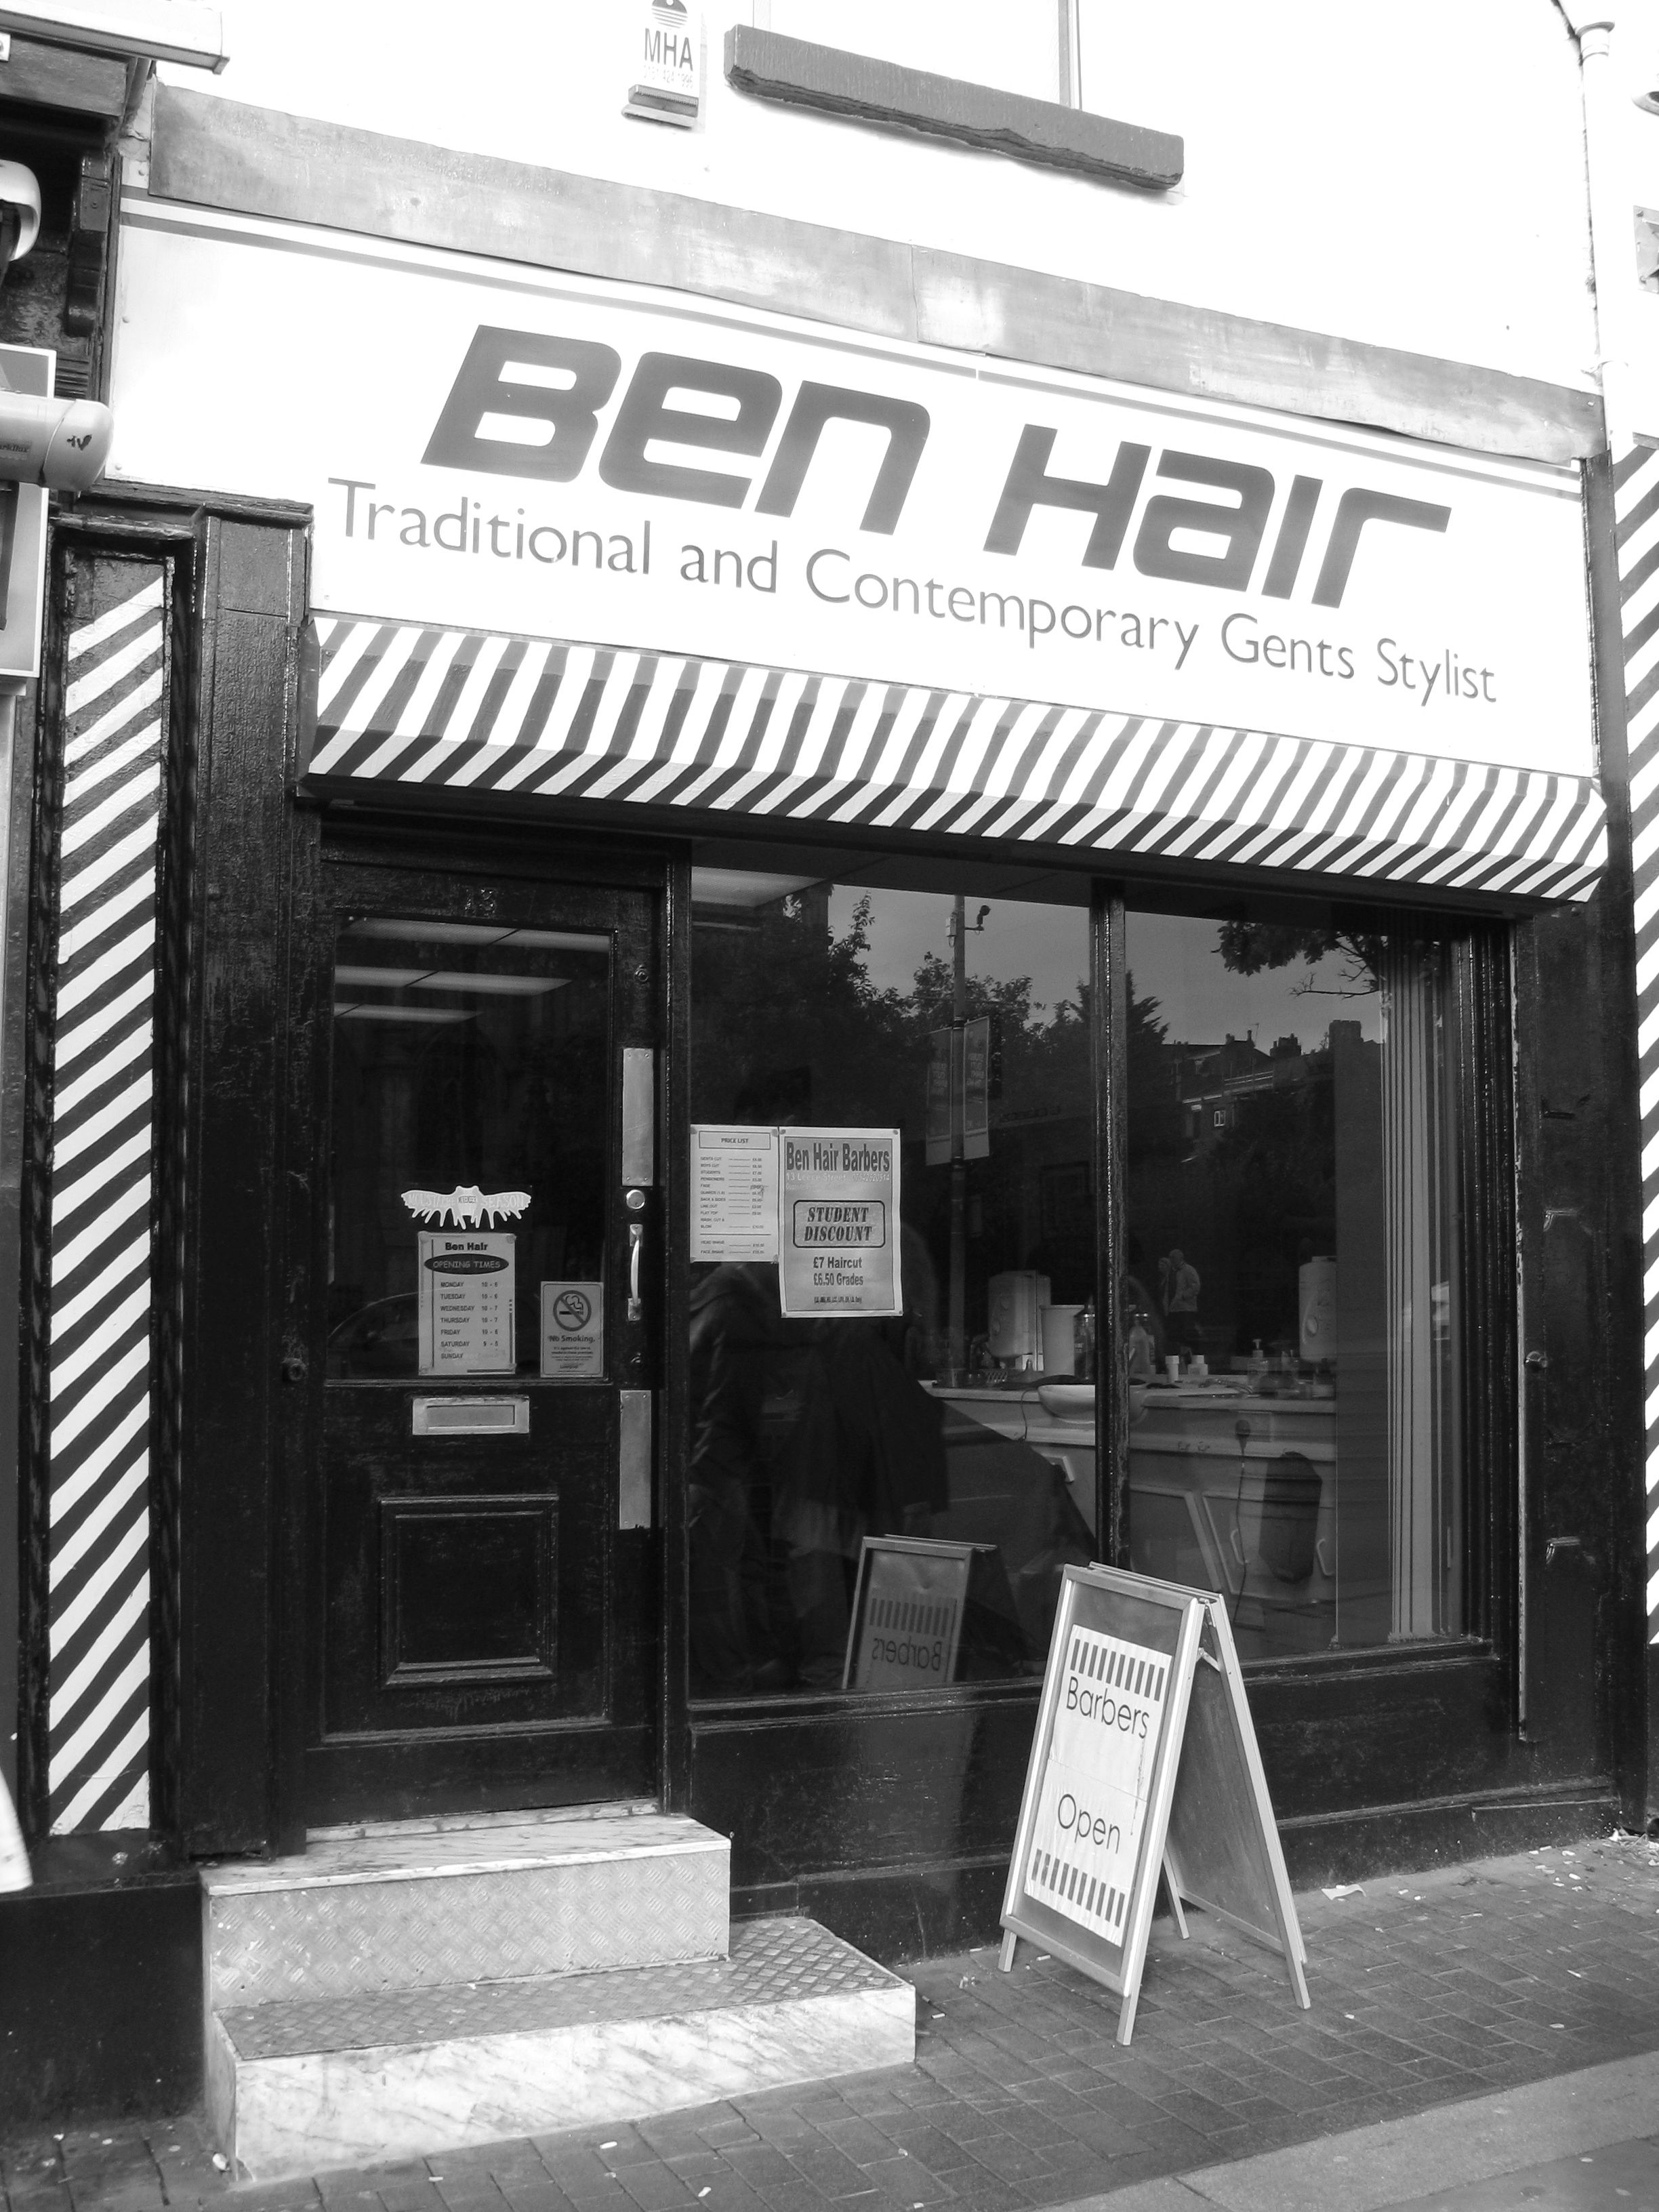
\includegraphics[width=\textwidth]{figures/benhair}
			\end{subfigure}
			\begin{subfigure}[h]{0.45\textwidth}
				
				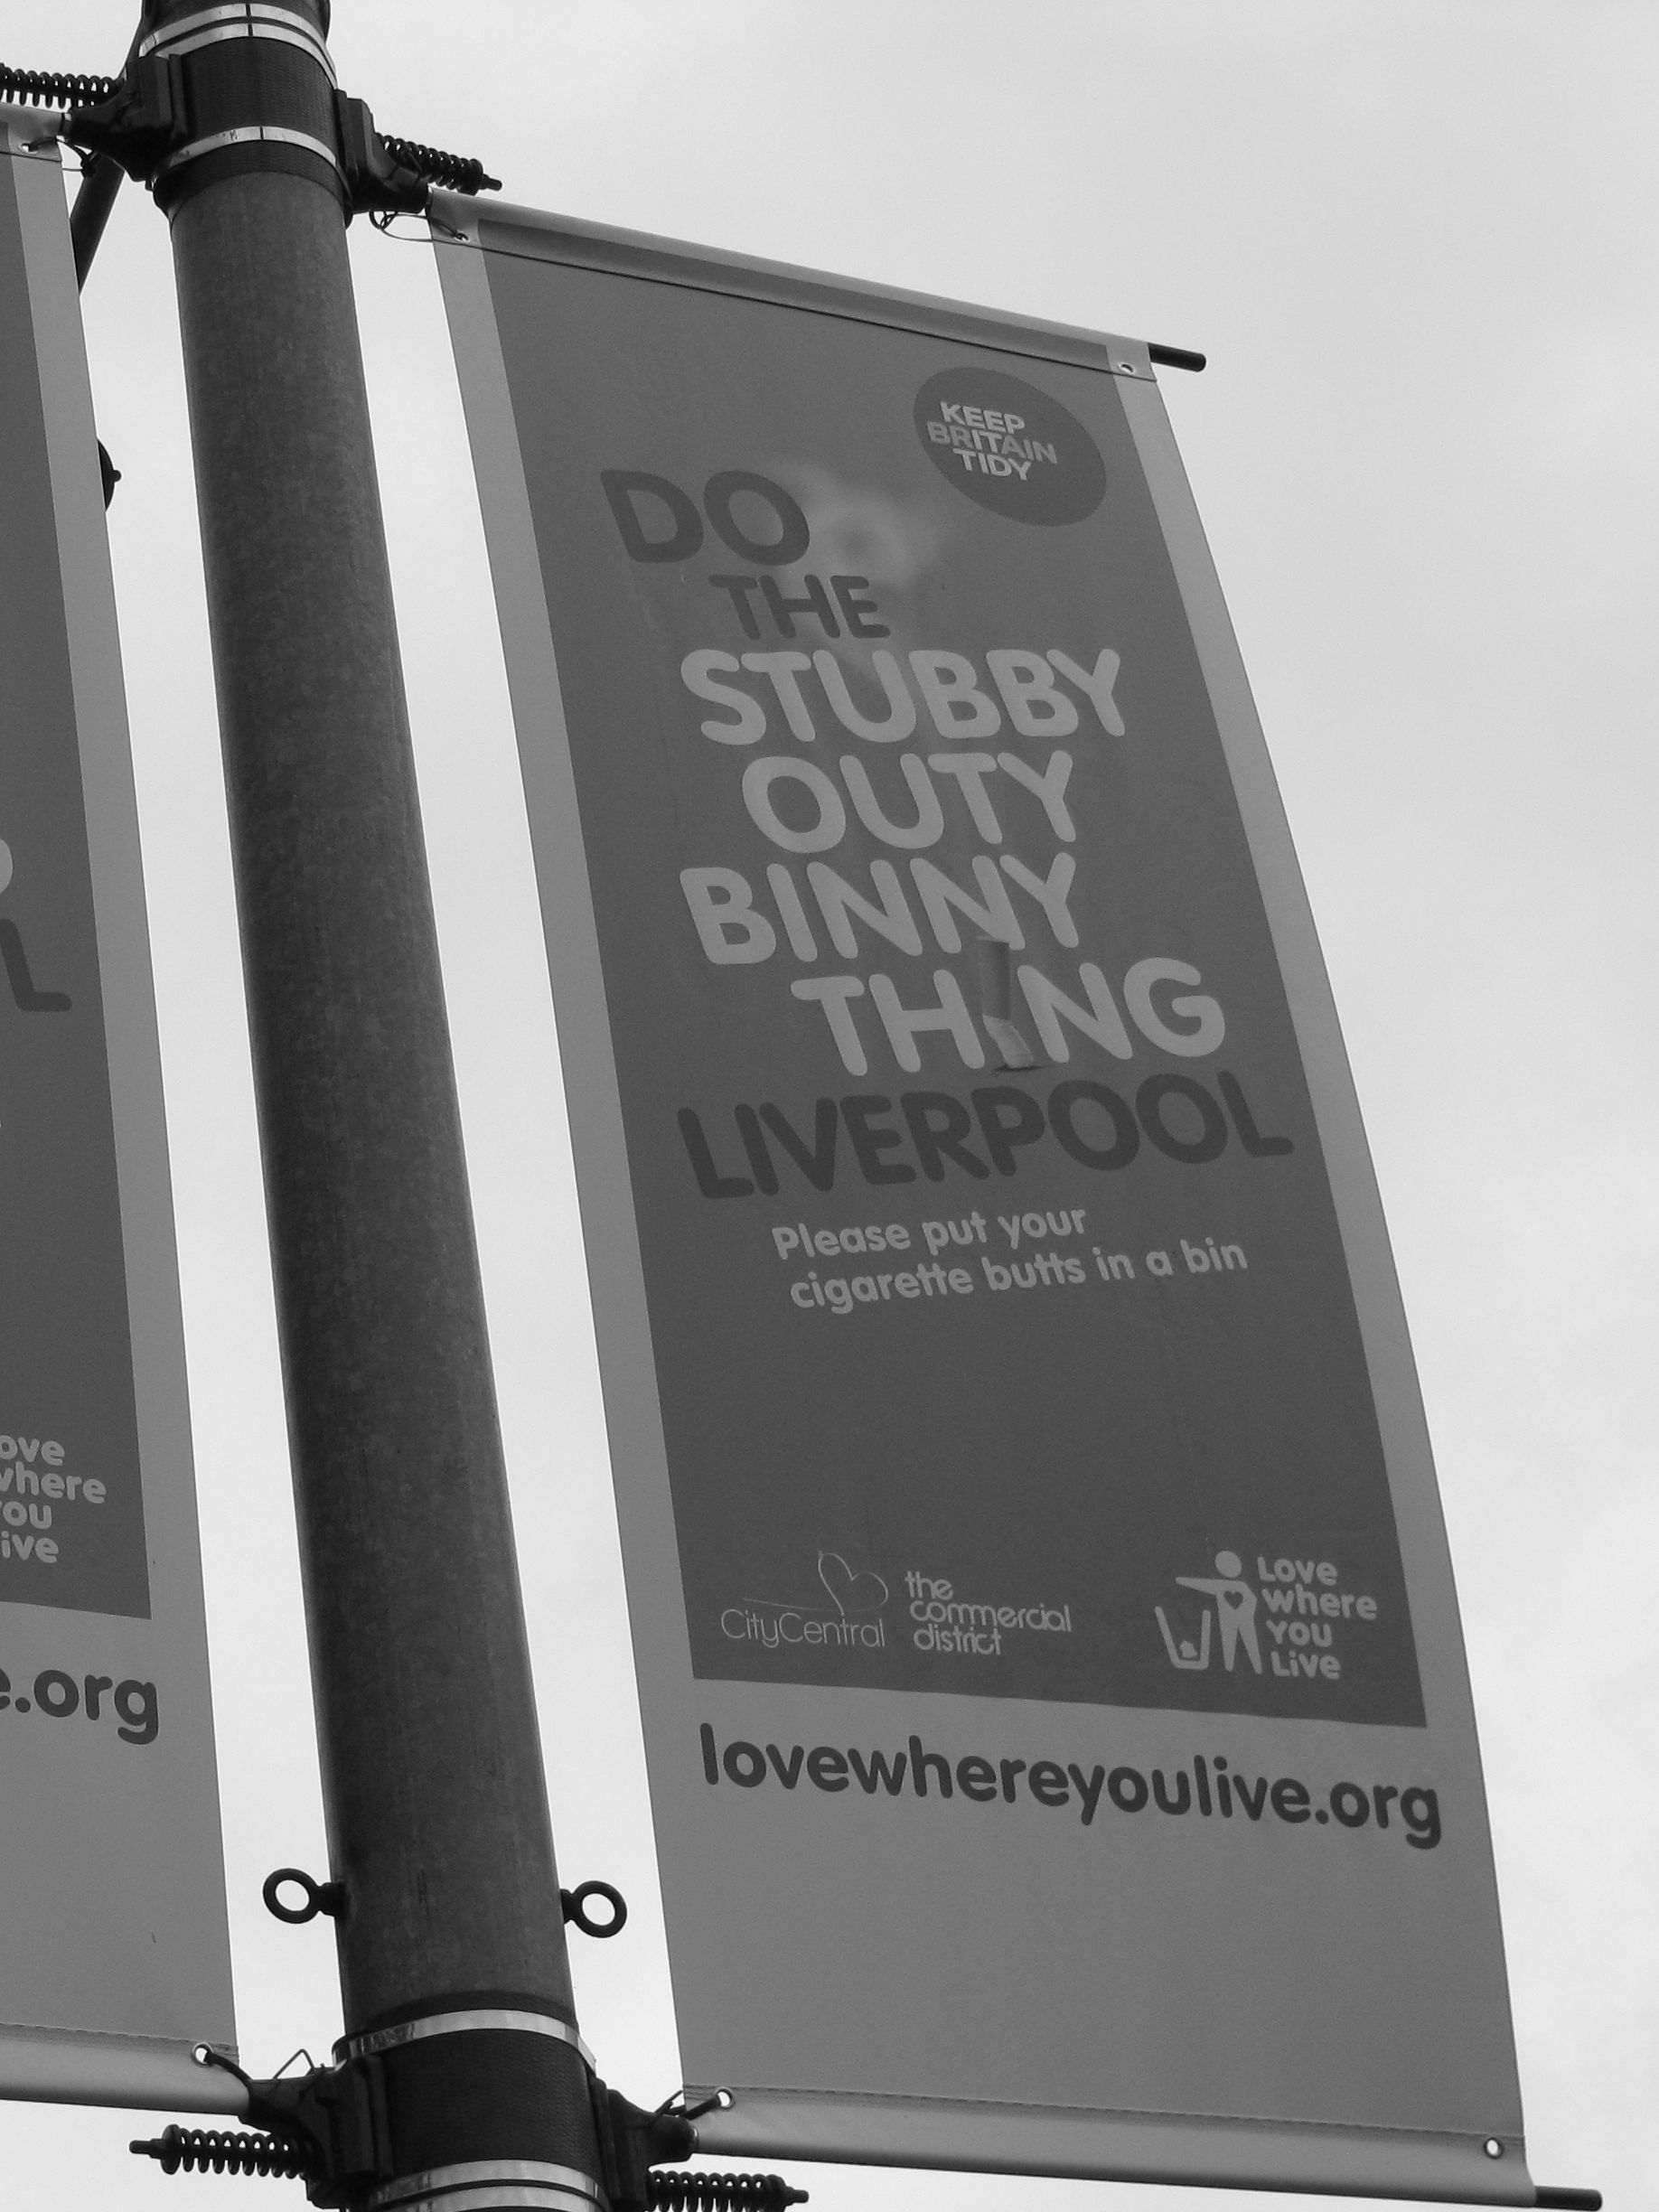
\includegraphics[width=\textwidth]{figures/stubby}
			\end{subfigure}
		\caption{Examples of enregisterment in Liverpool city centre}
		\label{fig.posters}
	\end{figure}

\section{Summary}\label{sec.hist.con}

We have seen how Liverpool developed from a tiny fishing village on the \isi{Lancashire} coast to a world centre of trade and commerce.
In the 19\textsuperscript{th} century, Scouse was formed when people from all over Britain and the Empire flocked to the city.
A hundred years later, Liverpool's long decline began and accelerated after World War 2 before it finally started to recover from the 1990s onwards and became a major tourist destination.
The city's external and internal \isi{image} followed suit.
Representations went from `Second city of the Empire' in the 19\textsuperscript{th} century to the extremely popular `Beat city' in the 1960s and then via the `Beaten city' of the Thatcher era to a more positive \isi{image} again linked to its year as European Capital of Culture.
Among other topics, this book will investigate whether the \isi{change}s in Liverpool's \isi{image} during the latter half of the last century (from positive to extremely negative to more positive again) have left their mark on the linguistic behaviour of Liverpudlians.